% !TEX encoding = UTF-8 Unicode
% !TEX root = main_org.tex
\chapter{Data analysis}
\section{Data selection}

In this chapter, we outline the selection criteria applied for this analysis. Basically, we used LHC10 data with pass 2 reconstruction which marked as ``good run". The period of data taking is LHC10h and it is only data sets from heavy ion collisions from 2010. 



\subsection{Default cuts and settings}
 
 The data sample recorded by ALICE during the 2010 heavy-ion run at the
LHC is used for this analysis. Detailed procedure of the ALICE
data taking can be found
in~\cite{Aamodt:2008zz,Carminati:2004fp,Alessandro:2006yt}. The Time
Projection Chamber (TPC) was used to reconstruct charged particle
tracks and measure their momenta with full azimuthal coverage in the
pseudo-rapidity range $|\eta|<0.8$. Two scintillator
arrays (V0) which cover the pseudo-rapidity ranges $-3.7<\eta<-1.7$
and $2.8<\eta<5.1$ were used for triggering, and the determination of
centrality~\cite{Aamodt:2010cz}. The trigger
conditions and the event selection criteria are identical to those
described in~\cite{Aamodt:2010pa, Aamodt:2010cz}.
Approximately $10^7$ minimum-bias Pb-Pb events with
a reconstructed primary vertex within $\pm 10$ cm from the nominal
interaction point in the beam direction are used for this
analysis. Charged particles reconstructed in the TPC in $|\eta|<0.8$
and $0.2<p_T<5$ GeV/$c$ were selected. The charged track quality cuts
described in~\cite{Aamodt:2010pa} were applied to minimize
contamination from secondary charged particles and fake tracks. The
charged particle track reconstruction efficiency and contamination
were estimated from {\sc HIJING} Monte Carlo
simulations~\cite{Wang:1991hta} combined with a {\sc
GEANT3}~\cite{Brun:1994aa} detector model, and found to be independent of
the collision centrality. The reconstruction efficiency increases from
70\% to 80\% for particles with $0.2<p_T<1$~GeV/$c$ and remains
constant at $80 \pm 5$\% for $p_T>1$~GeV/$c$. The estimated
contamination by secondary charged particles from weak decays and
photon conversions is less than 6\% at $p_T=0.2$~GeV/$c$ and falls
below 1\% for $p_T>1$~GeV/$c$.
With this choice of low $p_T$ cut-off ($p_T > 0.2$ GeV/$c$) we are reducing event-by-event biases from smaller reconstruction efficiency 
at lower $p_T$, while the high $p_T$ cut-off ($p_T < 5.0$ GeV/$c$) was introduced to reduce the contribution to the anisotropies from jet particles. 


The default estimator for centrality determination in ALICE is obtained from the measurement multiplicity in the VZERO detectors. 

\begin{center} \tiny{
\begin{tabular}{ |c|c c c c c c c c| } 
 \hline
Centrality(\%)&0-5      &5-10     &10-20    &20-30    &30-40     &40-50      &50-60      &60-70\\ 
\hline
b(fm) AMPT    &0.00-3.72&3.72-5.23&5.23-7.31&7.31-8.88&8.88-10.20&10.20-11.38&11.38-12.47&12.47-13.50\\ 
b(fm) HIJING  &0.00-3.60&3.60-5.09&5.09-7.20&7.20-8.83&8.83-10.20&10.20-11.40&11.40-12.49&12.49-13.49\\ 
b(fm) ALICE   &0.00-3.50&3.50-4.94&4.94-6.98&6.98-    &    -9.88 &9.81-      &     -12.09&12.09-\\
 \hline
\end{tabular}
\url{https://twiki.cern.ch/twiki/bin/viewauth/ALICE/CentStudies}
\label{table:impact} }
\end{center}



Also, even though the Inner tracking System (ITS) and the Time Projection Chanmber (TPC) were used as the main tracking devices for ALICE experiment, ITS does not have uniform acceptance. On the other hand, corrections for TPC are negligible due to its uniform acceptance. Because of this, we are going to use TPC only cuts in this analysis, in which the tracks are required to have at least 70 reconstructed space point out of the maximum 159 in the TPC and a $\langle \chi^2 \rangle$ per TPC cluster $\le 4$ (with 2 degrees of freedom per cluster)

Only tracks with a transverse distance of closest approach (DCA) to the primary vertex less than 3 mm
, both in longitudinal and transverse direction, are accepted to reduce the contamination from secondary tracks (for instance the charged particles produced 
in the detector material, particles from weak decays, etc.). 
Tracks with kinks (the tracks that appear to change direction due to multiple scattering, $K^{\pm}$ decays) were rejected.
 

\vskip20mm
\subsection{Data QA}

\subsubsection{ $\eta$ distribution QA} 

 In principle, the multiplicity in each $\eta$ region should be similar (i.e. $N_{Aside} \sim N_{Cside}$). To confirm this similarity of multiplicity in each $\eta$ set, we check $\eta$ distribution for each centrality bins. Also the multiplicity in $\eta < 0$ region  and $\eta > 0$ is compared as ratio. The ratio between number of multiplicity in $\eta>0 $ subgroup and $\eta<0$ subgroups,
was fitted with 0th order polynomial function with unity parameter(i.e $y=1$) run by run. After fitting, $\chi^2 / NDF$ was calculated to check for the same multiplicity in both subset groups for each run, each centralities.  Fig.\ref{dNdetaQA} are the $\eta$ distribution for run number 137135 and the $\chi^2/NDF$ test results over all run. The Run number corresponding Run ID information can be found in Appendix \ref{DataInfo}


	\begin{figure}[!hp]
		\begin{center}
        	\resizebox{0.45\columnwidth}{!}{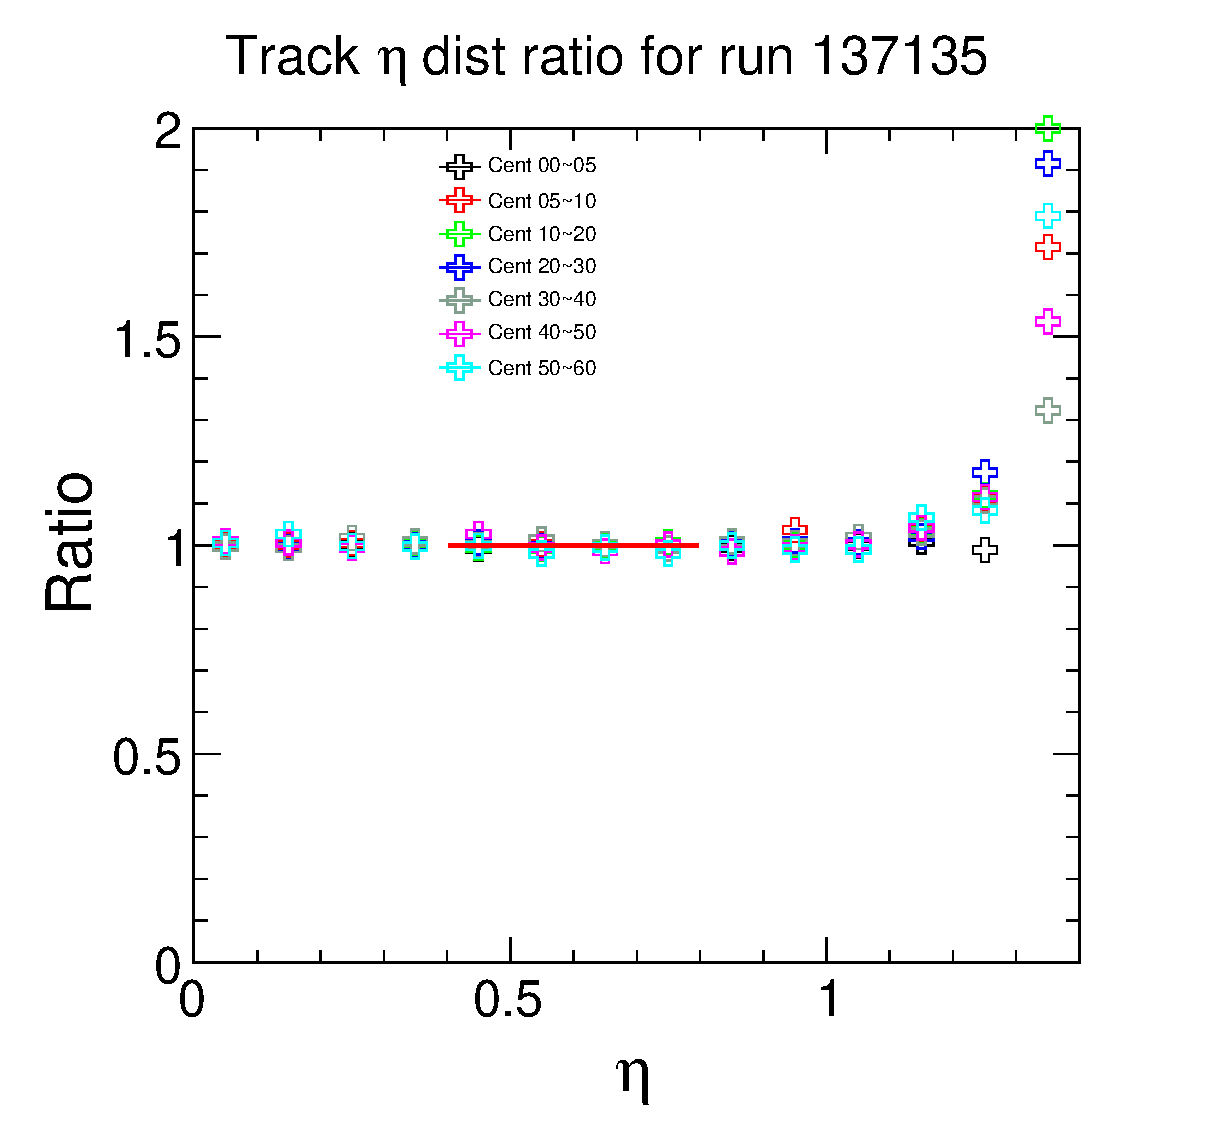
\includegraphics{figures/figs_QA/eta_ratio_run137135_eta_04_08.eps}}
	\resizebox{0.45\columnwidth}{!}{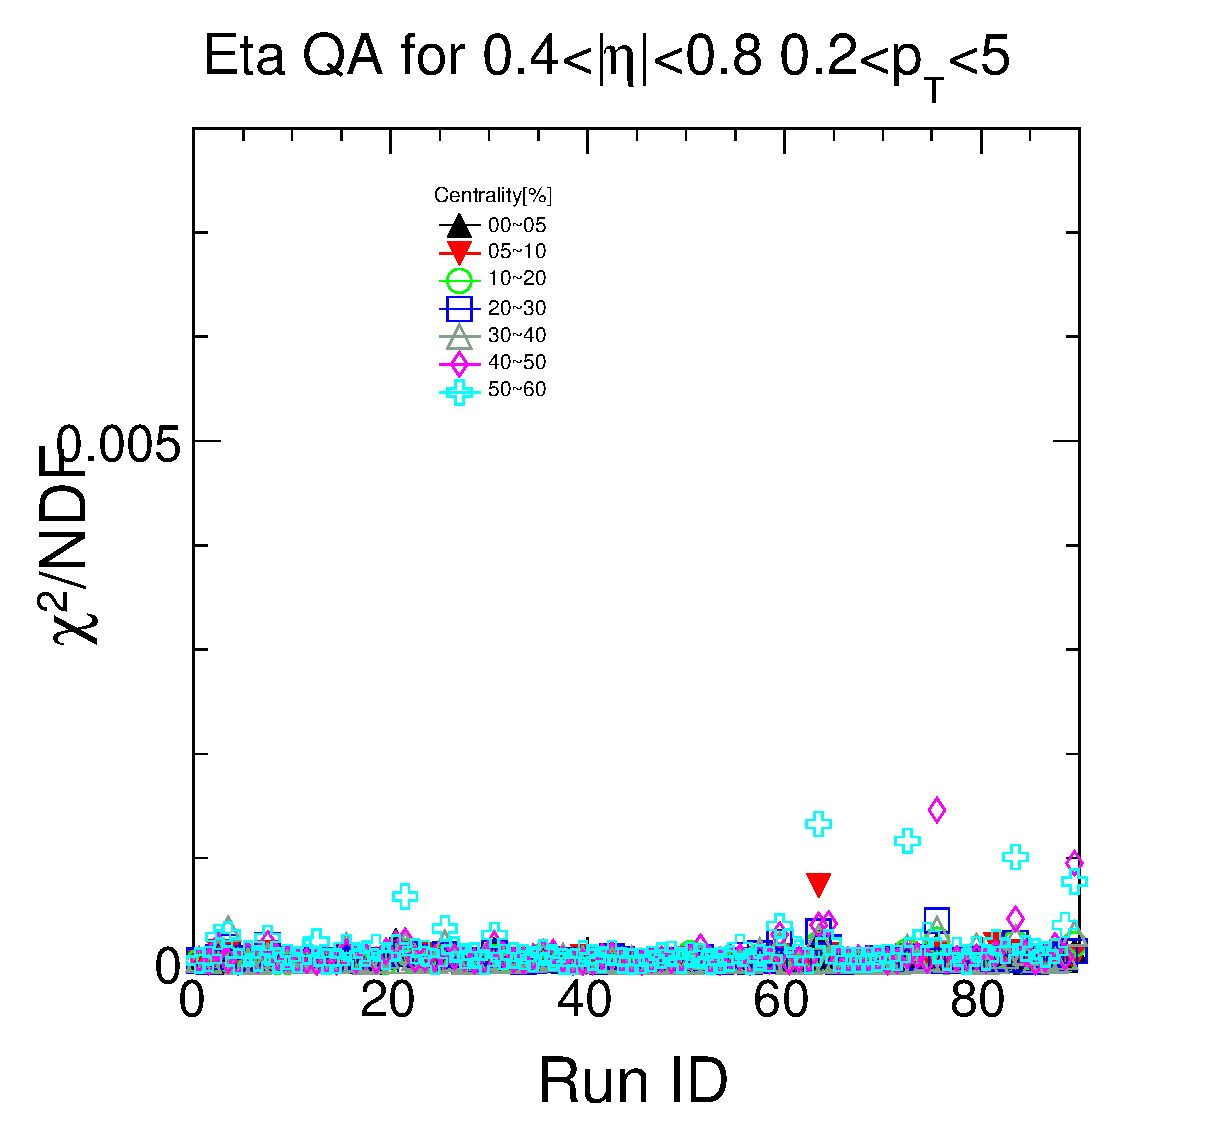
\includegraphics{figures/figs_QA/QA_Eta_ratio_flatness_LHC10h_AOD86.eps}}

        	\caption{Ratio of $dN/d\eta$ for flip over +/- $\eta$ region(left) and $\chi^2/NDF$ for $\phi$ flatness as function of RunID}
        	\label{dNdetaQA}
        \end{center}
    \end{figure}

QA result looks quite good across the runs as shown in figure. $\chi^2/NDF$ was lower than 0.002 for all runs and all centralities. As the results, we might simply assume that number of multiplicity in each subgroups are same.



\subsubsection{ $\phi$ distribution QA}

 $\phi$ flatness QA was performed on the $\phi$ distributions with the data. We fit the distributions with 0th-order polynomial. The distribution was fitted run by run. $\chi^2/NDF$ of each run were taken to estimate the flatness of distribution as like $\eta$ QA method. The fit results are shown in Fig.\ref{fig:QC_phi_chi2NDF}
 
    \begin{figure}[hp]
		\begin{center}
        	\resizebox{0.45\columnwidth}{!}{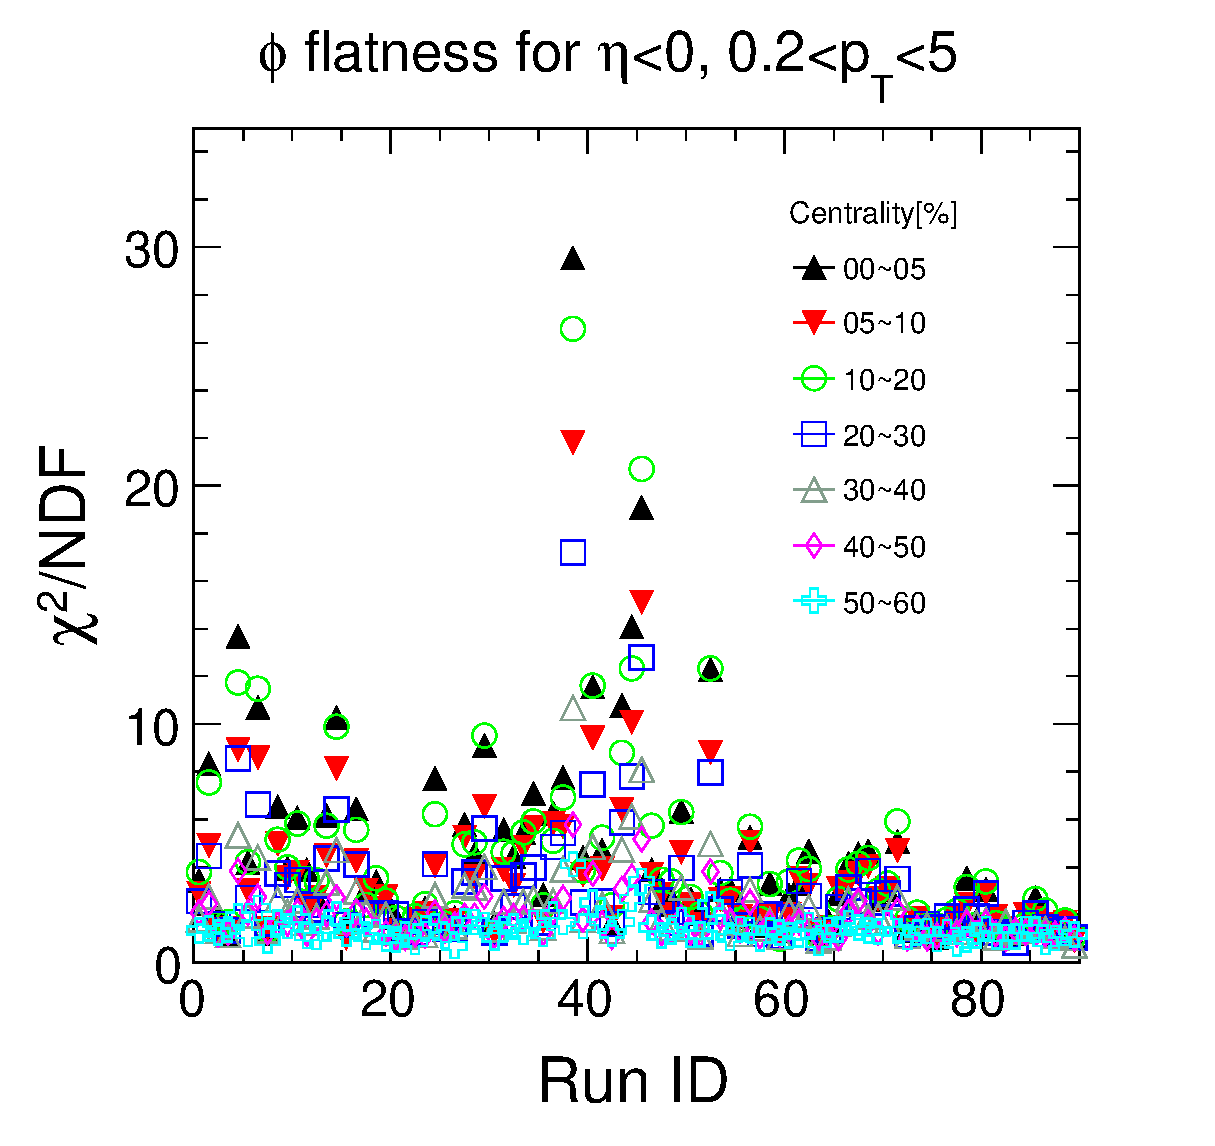
\includegraphics{figures/figs_QA/QA_RbR_phi_Aside_LHC10h_AOD86.eps}}
        	\resizebox{0.45\columnwidth}{!}{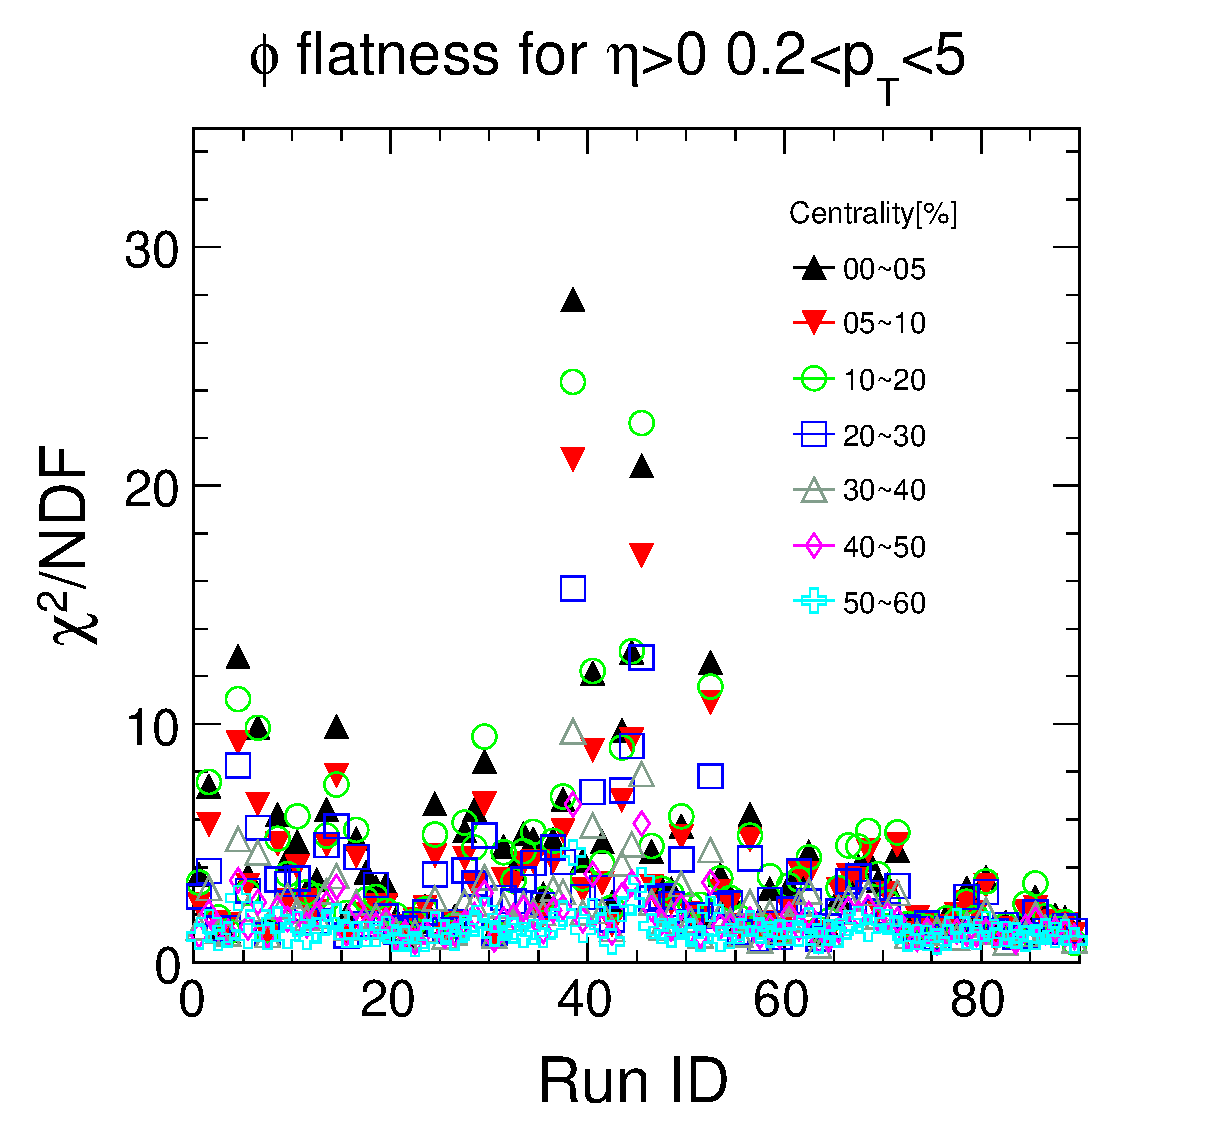
\includegraphics{figures/figs_QA/QA_RbR_phi_Cside_LHC10h_AOD86.eps}}
        \caption{$\chi^2/NDF$ for $\phi$ flatness for $\eta < 0$(left) and $\eta > 0$(right)}
        \label{fig:QC_phi_chi2NDF}
        \end{center}   
     \end{figure}

As shown in the figure, the flatness ($\chi^2/NDF$ of $\phi$) of some runs is worse than others. This is  considered as a detector effect, and might be affect on our analysis. The effect of these non-uniform $\phi$ distribution will be treated as systematics and will be covered in systematic chapter.
 

\clearpage

\section{Analysis strategy}
\label{sec:analysis}


While from existing measurements an estimate can be placed on the average value of QGP's $\eta/s$, both at RHIC and LHC energies, what remains completely unknown is how the $\eta/s$ of QGP depends on temperature ($T$). This study has been just initiated by the theorists in Ref.~\cite{Niemi:2015qia}, where the first (and only rather qualitative) possibilities where investigated (see Fig.~1 therein). The emerging consensus of late is that it is unlikely that the study of individual flow harmonics $v_n$ will reveal the details of $\eta/s(T)$ dependence. In fact, in was demonstrated already in the initial study~\cite{Niemi:2015qia} that different $\eta/s(T)$ parameterizations can lead to the same centrality dependence of individual flow harmonics. In Ref.~\cite{Niemi:2012aj} new flow observables were introduced by the theorists, which quantify the degree of correlation between two different harmonics $v_m$ and $v_n$. The initial success of these new observables was attributed to their potential to discriminate for the first time the two respective contributions to anisotropic flow development---from initial conditions and from the transport properties of the QGP~\cite{Niemi:2012aj}. Therefore their mesurement in turn would enable the experimental verification of theoretical predictions for individual stages of heavy-ion evolution independently. Besides this advantage, it turned out that correlations of different flow harmonics are sensitive to the details of $\eta/s(T)$ dependence~\cite{ALICE:2016kpq}, to which individual flow harmonics are nearly insensitive~\cite{Niemi:2015qia}. 

 For technical reasons, discussed in detail in Refs.~\cite{ALICE:2016kpq,Bilandzic:2013kga}, the correlations between different flow harmonics cannot be studied experimentally with the same set of observables introduced by the theorists in Ref.~\cite{Niemi:2012aj}. Instead, in~\cite{Bilandzic:2013kga} the new flow observables obtained from multiparticle correlations, so-called \textit{Symmetric Cumulants~(SC)}, were introduced to quantify in the most realiable way (i.e. nearly insensitivy to nonflow) the correlation of amplitudes of two different flow harmonics. The technical details are elaborated in Ref.~\cite{Bilandzic:2013kga}, while the first measurements of $SC$ observables were recently released by ALICE Collaboration in Ref.~\cite{ALICE:2016kpq}. For the convention, we will denote \textit{Symmetric Cumulants} for $m$th order and $n$th order as $SC(m,n)$ from now on.  This new observable are based on 4-particle cumulant, and defined as 

\begin{eqnarray}
	SC(m,n) &=&  \langle\langle \cos(m\varphi_1 + n\varphi_2 - m\varphi_3 - n\varphi_4 \rangle \rangle \nonumber \\ 
		&&- \langle \langle \cos{[m(\varphi_1 - \varphi_2)]} \rangle \rangle \langle \langle \cos{[n(\varphi_1 - \varphi_2)]} \rangle \rangle  \\ 
	  &=& \langle v_n^2 v_m^2 \rangle - \langle v_n^2 \rangle \langle v_m^2 \rangle \label{eq:SC}
\end{eqnarray}
\smallskip
 where double angular brackets indicates that the averaging has been extended from single to all events. Due to the condition that $m \neq n$, a lot of terms which appear in the general cumulant expansion are non-isotropic and  therefore, average to zero for a detector with uniform acceptance when the averaging is extended to all events. 
 
 
 These values can be obtained by multi-particle correlation with q-Cumulants such as 
 
\begin{equation}
	\langle \langle 2 \rangle \rangle \equiv \langle \langle e^{in(\phi_1 - \phi2)} \rangle \rangle \equiv \frac{\sum_{i=1}^{N}{(W_{\langle 2 \rangle})_i}\langle 2 \rangle_2 }{\sum_{i=1}^{N}{(W_{\langle 2 \rangle})_i}}
	\label{eq:2pcorr}
\end{equation}
\begin{equation}
	\langle \langle 4 \rangle \rangle \equiv \langle \langle e^{in(\phi_1 + \phi_2 - \phi_3 - \phi_4)} \rangle \equiv \frac{\sum_{i=1}^{N}{(W_{\langle 4 \rangle })_i}\langle 4 \rangle_i }{\sum_{i=1}^{N}{(W_{\langle 4 \rangle})_i}}
\end{equation}
\smallskip

The choice for the event weights in above equations is not arbitrary and we will outline in Appendix D. It has a physical meaning which will render the number of combinations (i.e. number of distinct 2- and 4-particle combinations one can form for an event with multiplicity M) as the only correct event weight.
 
 For fixed value of $v_n$ and $v_m$ over all events, the $SC(m,n)$ which defined as like Eq.\ref{eq:SC}, is zero by definition. Moreover we can obtain the result in the last line of above equation not only when $v_m$ and $v_n$ are fixed for all events, but also when event-by-event fluctuations of $v_m$ and $v_n$ are correlated( or anti-correlated).
 
This $SC(m,n)$ is very efficient observables for measuring flow ``magnitude" correlation because it's free from event-plane which is directly related to ``direction" correlation. (Any dependence on the event plane $\psi_n$ and $\psi_m$ is canceled by definition) 

As a result, the Eq.\ref{eq:SC} holds, the correlation between flow harmonics, and we can concluded whether finding $v_m$ larger than $\langle v_m \rangle$ in an event will enhance(or reduce) the probability of finding $v_n$ larger than $\langle v_n \rangle$ in that event. 

In this analysis, we are going to show $SC(m,n)$ results which can be calculated for correlation between flow harmonics by using 4- particle cumulants. In addition, we will show not only $SC(m,n)$ but also going to show  \textit{normalized} $SC(m,n)$ (also denote as $NSC(m,n)$)

\begin{eqnarray}
 NSC(m,n) &=& \frac{SC(m,n)}{\langle v_n^2 \rangle \langle v_m^2 \rangle } 	
 \label{eq:nSC}
\end{eqnarray}
\smallskip

\textit{Normalized symmetric cumulants} (NSC)  reflect only the degree of the correlation which is expected to be insensitive to the magnitudes of $v_{m}$ and $v_{n}$, while $SC(m,n)$ contains both the degree of the correlation and individual $v_{n}$ harmonics. In Eq.\ref{eq:nSC} the products in the denominator are obtained with two-particle correlations and using a psedorapidity gap of $|\Delta\eta|>1.0$ to suppress biases from few-particle nonflow correlations. On the other hand, in the two two-particle correlations which appear in the definition of $SC(m,n)$ the psedorapidity gap is not needed, since nonflow is suppressed by construction in \textit{SC observable}, as the study based on HIJING model has clearly demonstrated in Ref.~\cite{ALICE:2016kpq}.

However,  note that the following Eq.\ref{eq:nSC_1} and \ref{eq:nSC_2} are not held in this analysis because of the difference between products $\langle v_m^2 \rangle \langle v_n^2 \rangle$ for denominator and numerator. For the numerator, since nonflow is suppressed by construction in $SC(m,n)$ we do not apply any pseudorapidity($\eta$) gap for calculate 4- particle cumulants for all the particles in $|\eta| < 0.8$. But for the denominator, these products were obtained in ALICE with 2- particle correlations separately with using a pseudorapidity gap of $|\Delta \eta| >  1.0$ to suppress biases from few particle non-flow correlations. However, other theoretical studies \cite{Giacalone:2016afq} use both Eq.\ref{eq:nSC} and \ref{eq:nSC_2} for the  $NSC(m,n)$


\begin{eqnarray}
 NSC(m,n) &=& \frac{SC(m,n)}{\langle v_n^2 \rangle \langle v_m^2 \rangle } \nonumber \\ &=& \frac{ \langle  v_n^2 v_m^2 \rangle  - \langle v_n^2 \rangle \langle v_m^2 \rangle }{\langle v_n^2 \rangle \langle v_m^2 \rangle } \label{eq:nSC_1} \\ &=&   \frac{ \langle  v_n^2 v_m^2 \rangle   }{\langle v_n^2 \rangle \langle v_m^2 \rangle   }   -1	 \label{eq:nSC_2}
\end{eqnarray}


The $SC(m,n)$ provide orthogonal information to recently measured symmetry plane correlators in Refs.~\cite{ALICE:2011ab,Adare:2011tg,Aad:2014fla}. This statement does not exclude the possibility that both set of observables can be sensitive to the same physical mechanisms. In the recent theoretical study~\cite{Giacalone:2016afq} it was pointed out that the mechanism giving rise to symmetry plane correlations (nonlinear coupling) can also contribute to symmetric cumulants. As a concrete example it was discussed that the existing correlation due to hydrodynamic evolution between $V_4$ and $V_2^2$ (which are vectors in the transverse plane) implies that both the angles and the magnitudes are correlated~\cite{Giacalone:2016afq}. 

Interpretation of flow results obtained with multiparticle correlation techniques in small colliding systems, like pp and p--Pb at LHC, remains a challenge. The underlying difficulty stems from the fact that when anisotropic flow harmonic $v_n$ is estimated with $k$-particle correlator, the statistical spread of that estimate scales to leading order as $\sigma_{v_{n}}\sim\frac{1}{\sqrt{N}}\frac{1}{M^{k/2}}\frac{1}{v_{n}^{k-1}}$, where $M$ is the number of particles in an event (multiplicity) and $N$ is total number of events. This generic scaling ensures that multiparticle correlations are precision method only in heavy-ion collisions, characterized both with large values of multiplicity and flow. To leading order the measurements in small systems~\cite{Aad:2013fja,Abelev:2014mda,Khachatryan:2015waa,Adamczyk:2015xjc,Adare:2015ctn} and the measurements in heavy-ion collisions resemble the same features, which can be attributed to collective anisotropic flow in both cases. However, such interpretation is challenged by the outcome of recent Monte Carlo study~\cite{Loizides:2016tew} for $e^+e^-$ systems in which collective effects are not expected. Nonetheless, in this study to leading order multiparticle correlations exhibit yet again the similar universal trends first seen in heavy-ion collisions, both for elliptic and triangular flow. Therefore, it seems unlikely that the analysis of individual flow harmonics with multiparticle techniques will answer whether collective effects can develop and QGP be formed in small systems---instead new observables, like SC, might provide the final answer due to their better sensitivity~\cite{Niemi:2012aj,ALICE:2016kpq}.



\subsubsection{Measuring $SC(m,n)$ with Scalar Product method}
In this analysis, we are going to show that $SC(m,n)$ also can be calculated  by the Scalar Product(SP) method via measuring moments \cite{Bhalerao:2015jg} with single $\eta$ gap. By introducing single $\eta$ gap between two different sub-event group can avoid auto (self)-correlation and can suppress non-flow effects. To calculate SC(m,n) with the SP method, we need to define the (normalized) flow Q-vector such as

\begin{equation}
	 Q_n = \frac{1}{N} \sum{e^{in\varphi}  } 
\end{equation}

Then, the flow magnitude can be easily obtained with $Q$-vector calculation. 

\begin{equation}
	\langle v_n^{2k} \rangle  = \langle V_n^{k*} V_n^k\rangle= \langle Q_{nA}^{*k} Q_{nB}^k \rangle
\end{equation}

To avoid self-correlation when calculating $v_n^2$, we divide particles into 2 sub event groups and introduced single $\eta$ gap between sub event group to suppress non-flow effect. So main difference between original method and this method is that calculate correlation with full-particle $Q$-vector or divided-particle $Q$-vector, and existence of $\eta$ gap around 0. 

\begin{eqnarray}
\langle v_m^2 v_n^2 \rangle - \langle v_m^2 \rangle \langle v_n^2 \rangle 
 &=& \langle V_n V_n^{*} V_m V_m^{*}\rangle - \langle V_n^k V_n^{*} \rangle \langle V_m^k V_m^{*}\rangle \\ 
 &=& \langle {Re( Q_{An} Q_{Bn}^* Q_{Am} Q_{Bm}^*)} \rangle - \langle {Re( Q_{An}Q_{Bn}^*) } \rangle  \langle { Re(Q_{Am} Q_{Bm}^*) }\rangle \nonumber \\  
\end{eqnarray}


In this analysis, we take denotation ``A" for sub-event group which have negative $\eta$ range ( $-0.4 > \eta > -0.8$ ) and ``B" for positive $\eta$ range ( $0.4 < \eta < 0.8$ ). Because we divided into 2 sub groups, particles will not count twice when calculating $Q_{An} Q_{Bn}^*$, but there are still possible of auto (self) correlation when calculating ``$Q_{An} Q_{Bn}^* Q_{Am} Q_{Bm}^*$", this effect is probably small but can be corrected with the analytical method. 

\begin{equation}
	v_n^{2k}v_m^{2l} = \langle  Q_{nA}^{*k} Q_{nB}^k Q_{mA}^{*k} Q_{mB}^k \rangle
\end{equation}

The auto correlation during above the equation happens because there is a $\eta$ gap between $Q_{nA}^{*k} Q_{nB}^k$, and $Q_{mA}^{*k} Q_{mB}^k$ but not between $Q_{nA}^{*k}Q_{mA}^{*k}$ nor $Q_{nB}^k Q_{mB}^k$,  the auto (self) correlation effect can be corrected by changing equation of $SC(m,n)$ from

\begin{equation}
	\langle {Re( Q_{An} Q_{Bn}^* Q_{Am} Q_{Bm}^*)} \rangle - \langle {Re( Q_{An}Q_{Bn}^*) } \rangle  \langle { Re(Q_{Am} Q_{Bm}^*) }\rangle 
\end{equation}
to

\begin{equation}
\begin{split}
	\langle &Re( Q_{An} Q_{Bn}^* Q_{Am} Q_{Bm}^*) - \frac{1}{M_B} Re(Q^*_{Bm+n}Q_{Am}Q_{An})\\
	 &-\frac{1}{M_A}Re(Q_{Am+n}Q^*_{Bn}Q^*_{Bm}) + \frac{1}{M_A M_B}Re(Q_{Am+n}Q^*_{Bm+n}) ) ) \rangle  \\
	 &- \langle {Re( Q_{An}Q_{Bn}^*) } \rangle  \langle { Re(Q_{Am} Q_{Bm}^*) }\rangle
\end{split}		
\end{equation}

	\begin{figure}[h]
		\begin{center}
     	   	\resizebox{0.45\columnwidth}{!}{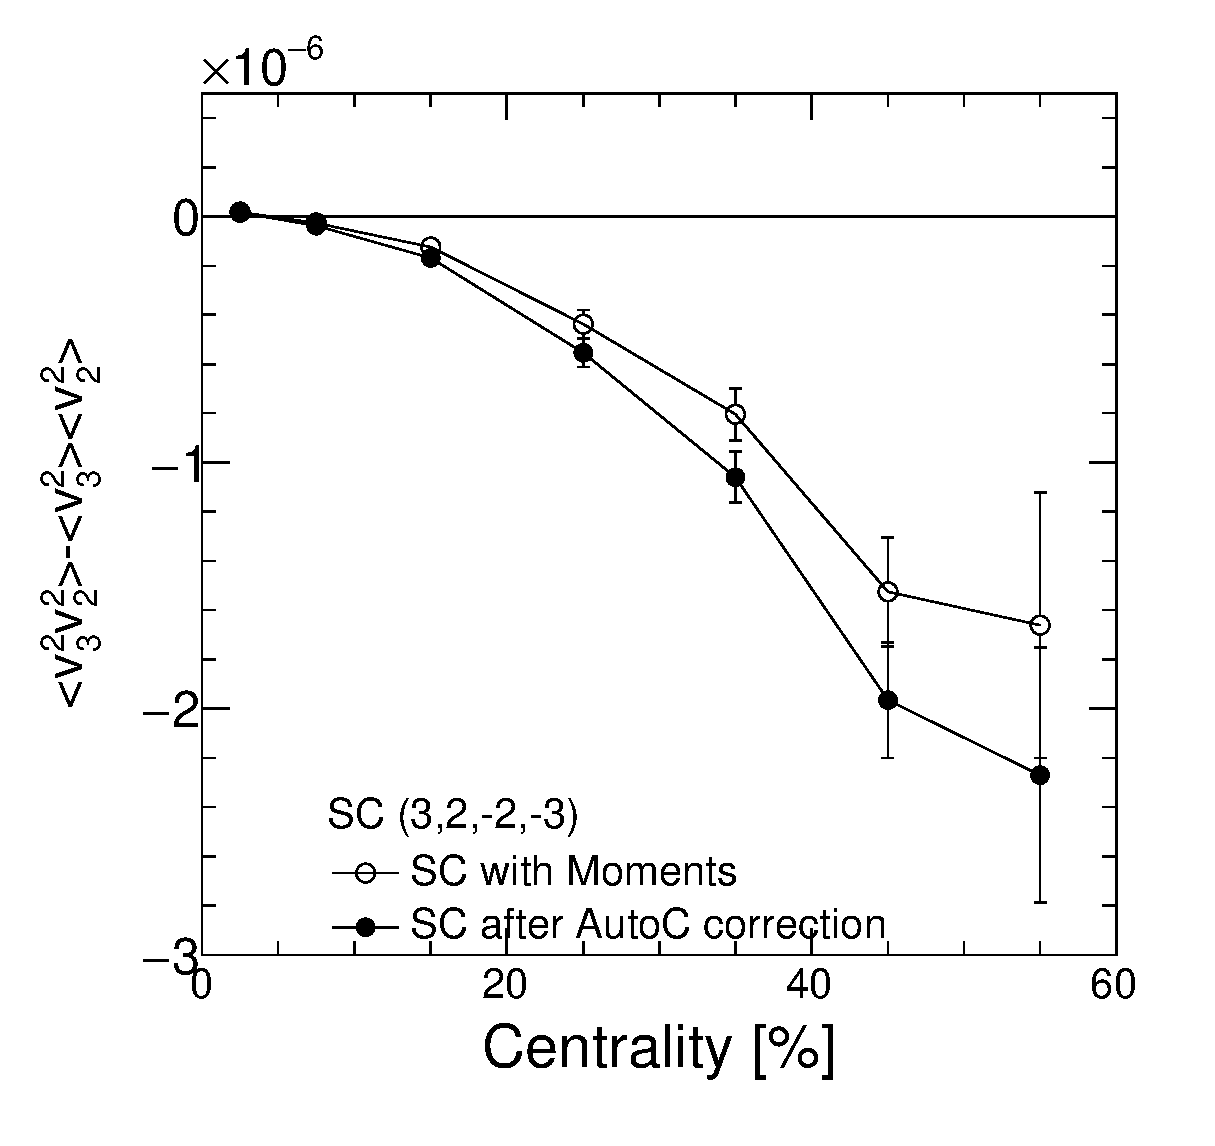
\includegraphics{figures/figs_SCpt/SC_LHC10h_3223_compare}}
              	\resizebox{0.45\columnwidth}{!}{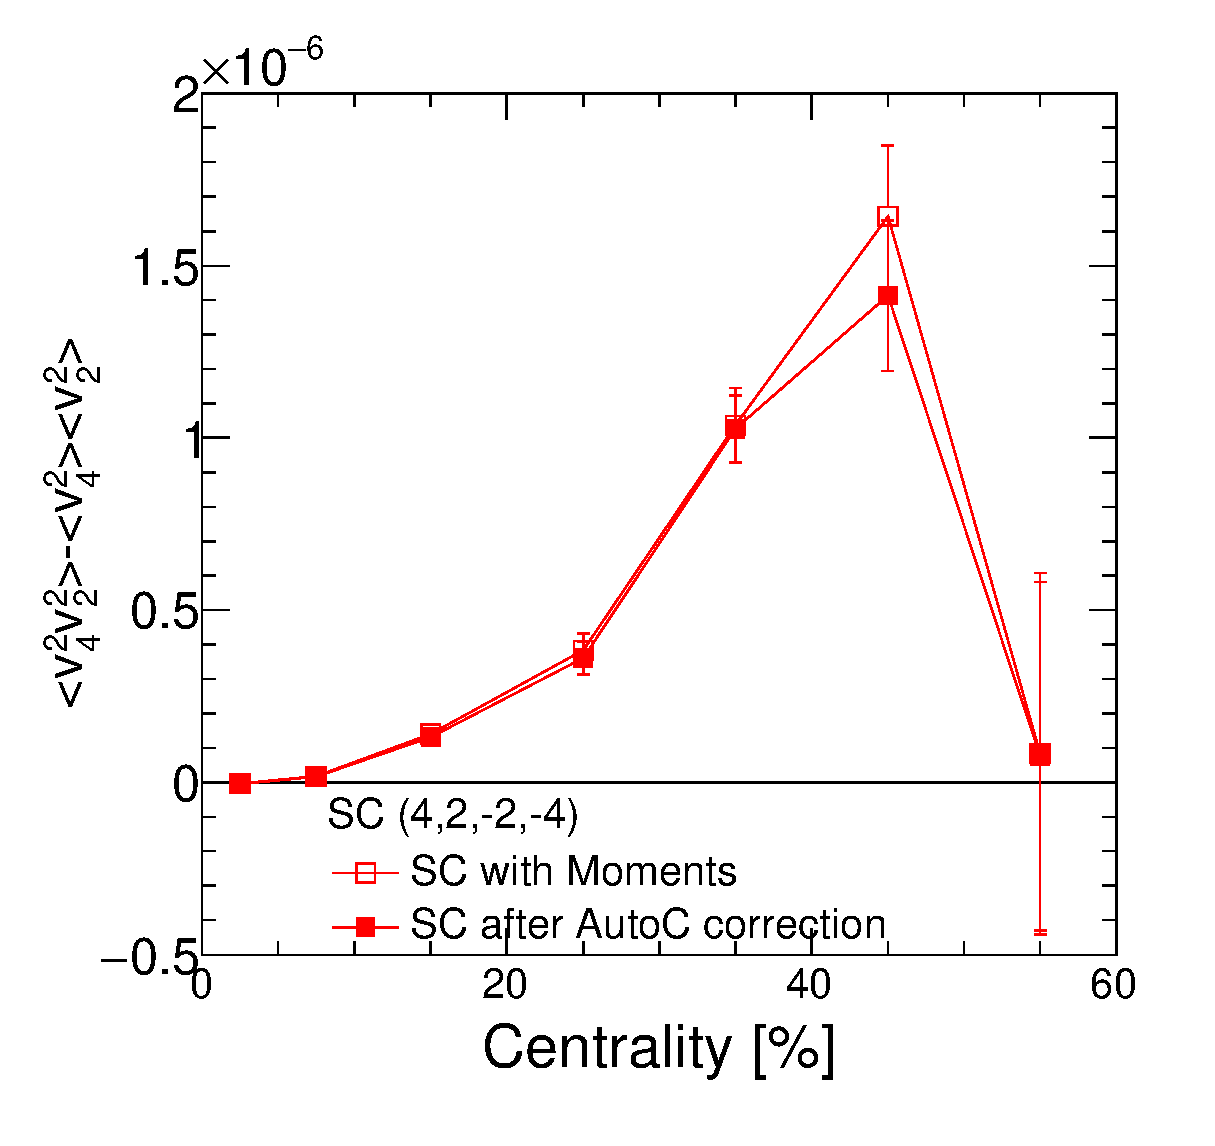
\includegraphics{figures/figs_SCpt/SC_LHC10h_4224_compare}}
        \label{SC42_autoC}
        \caption{Results of $SC(3,2)$(left) and $SC(4,2)$ before auto (self)-correlation correction(open makers) and after correction(closed markers)}
        \end{center}   
     \end{figure}




\vskip15mm

The detailed results of $SC(m,n)$ and  $NSC(m,n)$ with various flow harmonics, and comparison with hydrodynamic calculations and MC simulations, and also the $p_T$ dependence of $SC(m,n)$ and $NSC(m,n)$ and the difference between two different measuring method (QC vs SP) will be covered in the results chapter.

\section{Systematics}

	In this section, the systematic uncertainties of $SC(m,n)$ and  $NSC(m,n)$ will be presented. The systematic uncertainties were estimated by varying the event and track selection criteria. All systematic checks described here are performed independently. Each results of $SC(m,n)$ (and also $NSC(m,n)$) with a selected criterion are compared to ones from the default event and track selection described in the previous chapter. The differences between the default results and the ones obtained from the variation of the selection criteria are taken as systematic uncertainty of each individual source.
The different ratio were fitted with a 0-th order polynomial as function of centrality to suppress point-to-point statistical fluctuations and to extract the overall systematics. The contributions from different sources were then merged in quadrature to obtain the final value of the systematic uncertainty. The detailed conditions varying for systematics studies were described in the following.
	
	
	
\subsection{Systematics from Non uniform phi distribution}
	
	
This section is about systematics uncertainty from the non-uniform efficiency of detector performance. In principle, the $\phi$ distribution of produced particle should be flat over all events unless detector effect. But in our data, as seen in the previous section in data QA (see figure.\ref{fig:QC_phi_chi2NDF}), the distribution of the transverse angle of particle produced is not perfectly uniform due to detector effects like inefficiency or dead-zone area. And these non-uniform $\phi$ distributions vary run-by-run, and it is not easily corrected by simple weight correction for specific $\phi$ angle.

 This non-uniform $\phi$ distribution might change the final results of $SC(m,n)$ and should be taken into systematic uncertainty. The simplest and basic approach to check the effect of non-uniform distribution is categorize run groups into two sub groups to have good $\phi$ distribution, and for the other group to have bad $\phi$ distribution. Then measure the $SC(m,n)$ values with each sub groups independently and calculated the difference between them as the systematic uncertainty. However, to use this methods, we need to have almost same number of events for each groups. Even though we have similar number of events for each groups, we are going to have larger statistical error because of half of events in this way. 

  In this analysis, to check systematic uncertainties from non-uniform $\phi$ distribution, we use AMPT simulation which has better match to data than any other existing models. We measure $SC(m,n)$ with the large statistics AMPT dataset which has  flat $\phi$ distribution, and impose non-uniform $\phi$ distribution from data and calculate the difference between original AMPT and modified AMPT as systematic uncertainty from non-uniform $\phi$ distribution. 


 	\begin{figure}[h]
		\begin{center}
        	\resizebox{0.85\columnwidth}{!}{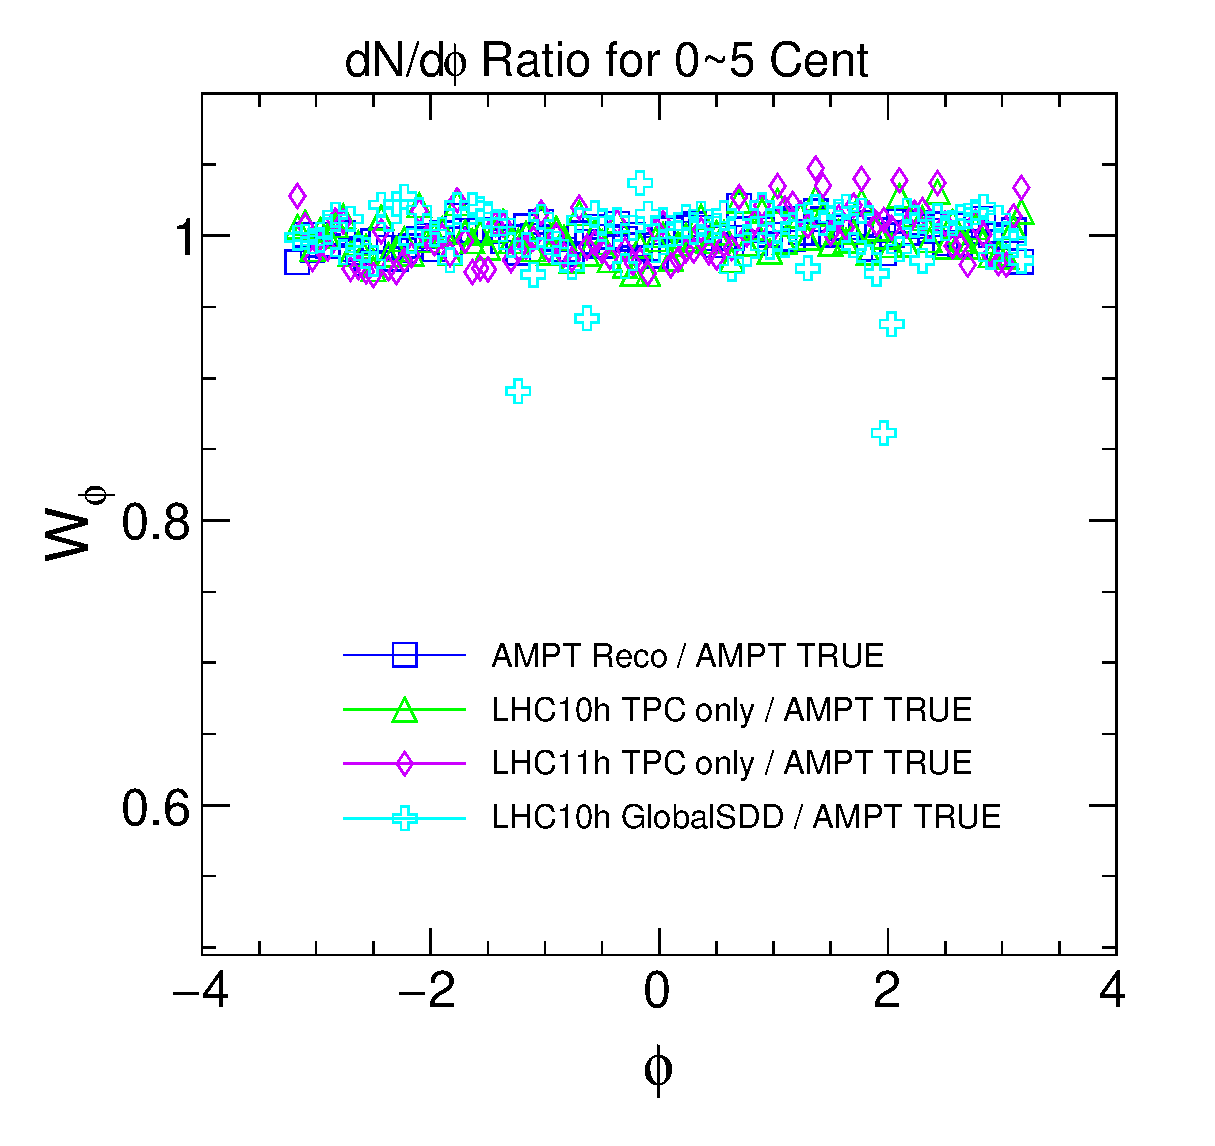
\includegraphics{figures/figs_QA/impose_NUE.eps}}
        \caption{Scaled ratio of $dN/d\phi$ distribution of ALICE LHC10h dataset to flat distribution (AMPT True). The reconstructed AMPT, and LHC11h with TPC only track cut, and LHC10h with Global SSD track cut were also drawn together for comparison.}
        \label{fig:QC_impose}
        \end{center}   
     \end{figure}
	
The non-uniform $\phi$ distribution which is taken from ALICE LHC10h data are shown in Fig.\ref{fig:QC_impose}. We use TPC only track cut, which have better $\phi$ distribution, but also LHC10h with Global SDD and LHC11h distribution were shown together for comparison. As seen in figure, the data from LHC10h period have worse flatness than AMPT simulation. It becomes even worse in GlobalSSD track cut or LHC11h period data because of some detector problems. (Some of SDD clusters in ITS detector were dead in 2010, and there was reconstruction efficiency issue with TPC detector in 2011 data taking) The results with AMPT data and modified AMPT data were calculated together and the difference between them was taken into systematic uncertainties. 


	\subsection{Systematics from Event selection}
	
	Following is the list of item for systemic uncertainty study about event selections. 
	
\subsubsection{Z-vertex cut}

Because of limited acceptance of ALICE detector, primary vertex position along the longitudinal direction is important to ensure for the uniform pseudo-rapidity distribution over all events. The z-vertex distribution of ALICE LHC10h events are shown in Fig.\ref{fig:zvtx}.  As described in previous chapter, the reconstructed vertex position in beam axis (z-vertex) is required to be located within 10 cm of interaction point (IP). Since  the different z-vertex position may have an effect on effective $\eta$ range. So these Z-vertex cut criteria are important to ensure for the flat $\eta$ distribution over all events. 	Instead of using the original vertex range cut ($|z| < 10$ cm),  we tried to reduce $|z| < 8$ cm for systematic study.	
		
 	\begin{figure}[h]
		\begin{center}
        	\resizebox{0.65\columnwidth}{!}{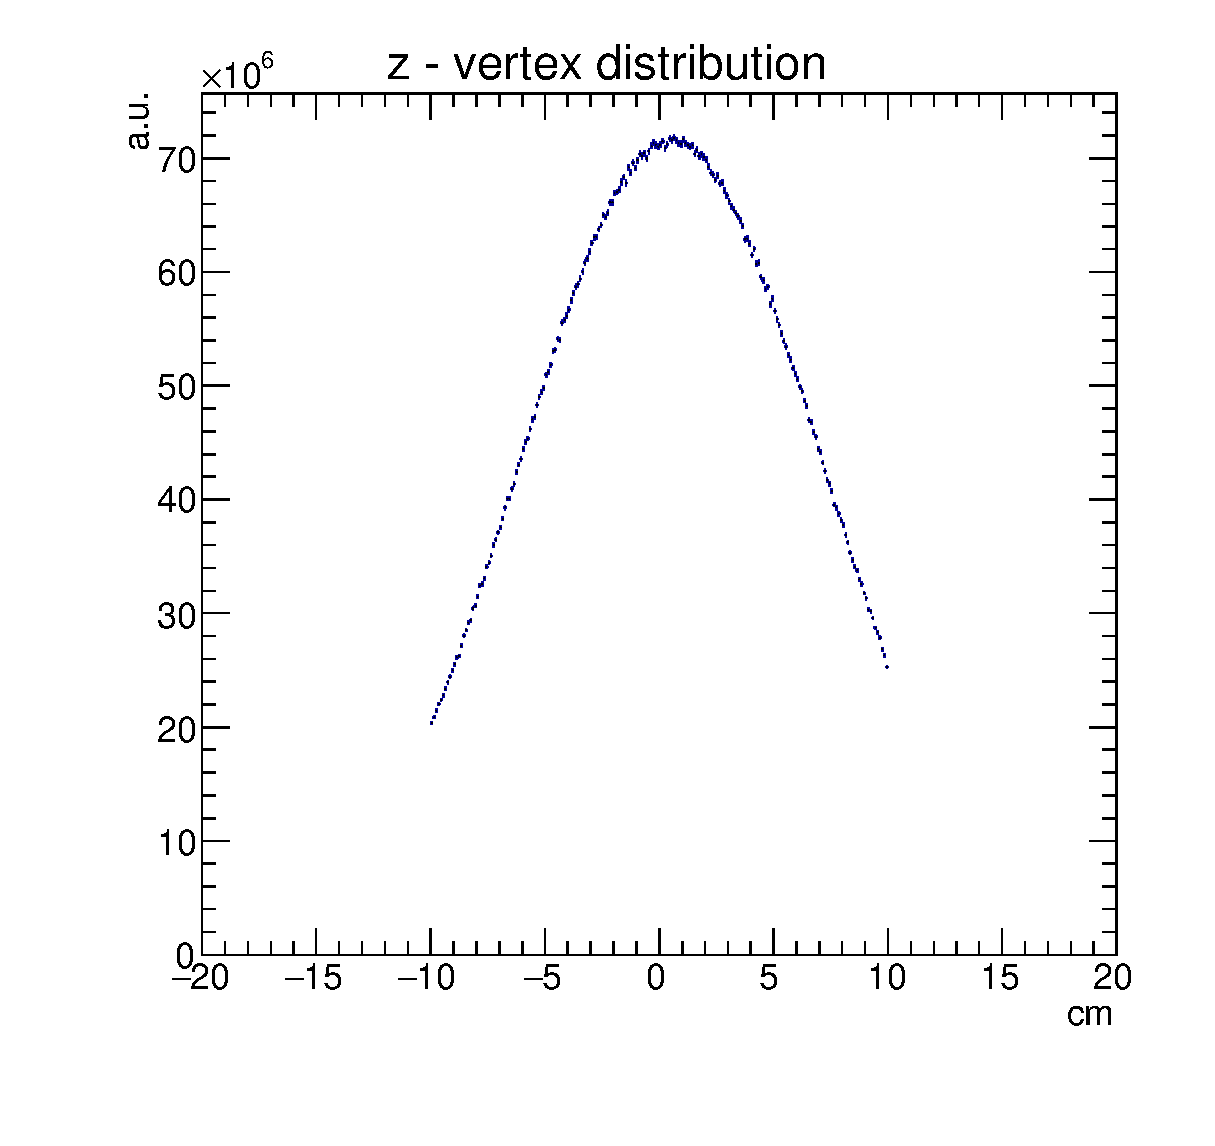
\includegraphics{figures/figs_systematics/zvtx_dist}}
        \caption{Z-vertex distribution of ALICE Pb + Pb $\sqrt{S_{NN}} = 2.76$~TeV with minimum bias triggered events }
        \label{fig:zvtx}
        \end{center}   
     \end{figure}


	
\subsubsection{Magnetic polarization}
	The events which we analyzed were recorded with two settings of the magnetic field polarities, namely (++) and  (--). For the default, we used all the events from both polarized magnetic fields. The configuration of magnetic polarizations consist of almost the same number of events. We measured the $SC(m,n)$ results from (++) or (--) categorized events and compare to the default one.
	
\subsubsection{Centrality determination}
	The centrality of the given collision can be determined by various detectors and settings. By the default, the multiplicity of the VZERO detector(Both V0A and V0C) is used for centrality determinations with better than 2\% of resolution. Another method of determine event centrality were using the multiplicity of tracks estimated by the standalone TPC tracking or tracklet from SPD detector independently which have slightly worse resolution. We use these methods to study systematic uncertainty from centrality determination.
	
\subsubsection{Cut on outliers}
	The outlier is an observation point that is different from other observations. In LHC10h datasets, there are some events which have many more TPC tracks than Global reconstructed tracks. These outliers is coming from pile-up like events or indicate experimental error. These kind of outliers usually are discarded from the data sets. In these case, we excluded the events which have Multiplicity of TPC except following criteria	
	
	\begin{equation}
		32.1 + 1.59 \times M_{Global} < M_{TPC} < -40.3 + 1.22 \times M_{Global} 
	\end{equation}
	
		
 	\begin{figure}[h]
		\begin{center}
        	\resizebox{0.45\columnwidth}{!}{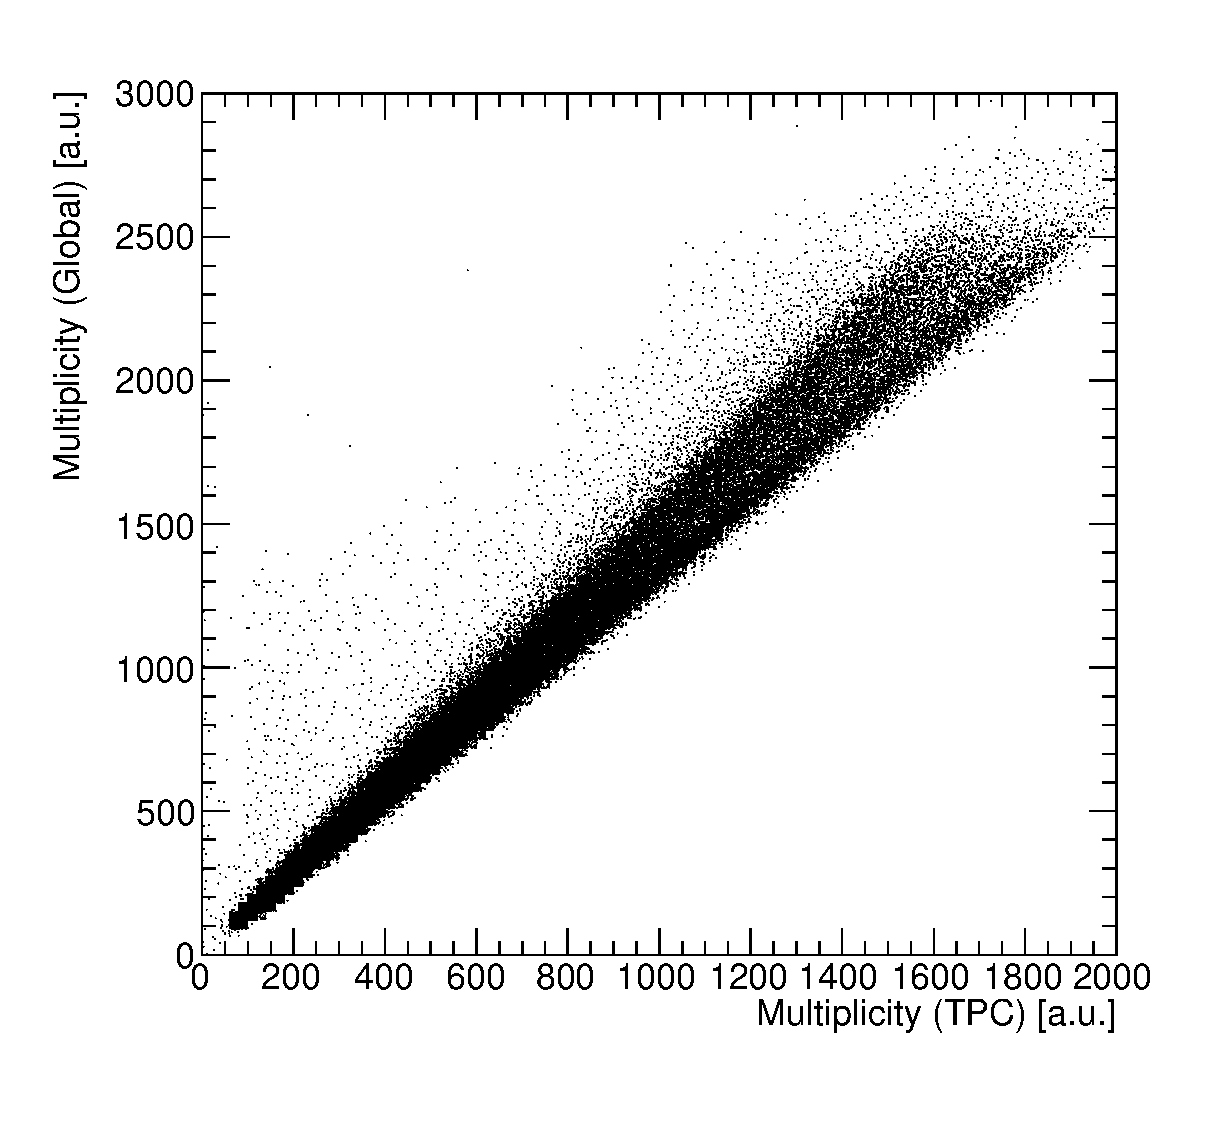
\includegraphics{figures/figs_systematics/outlier_off.eps}}
        	\resizebox{0.45\columnwidth}{!}{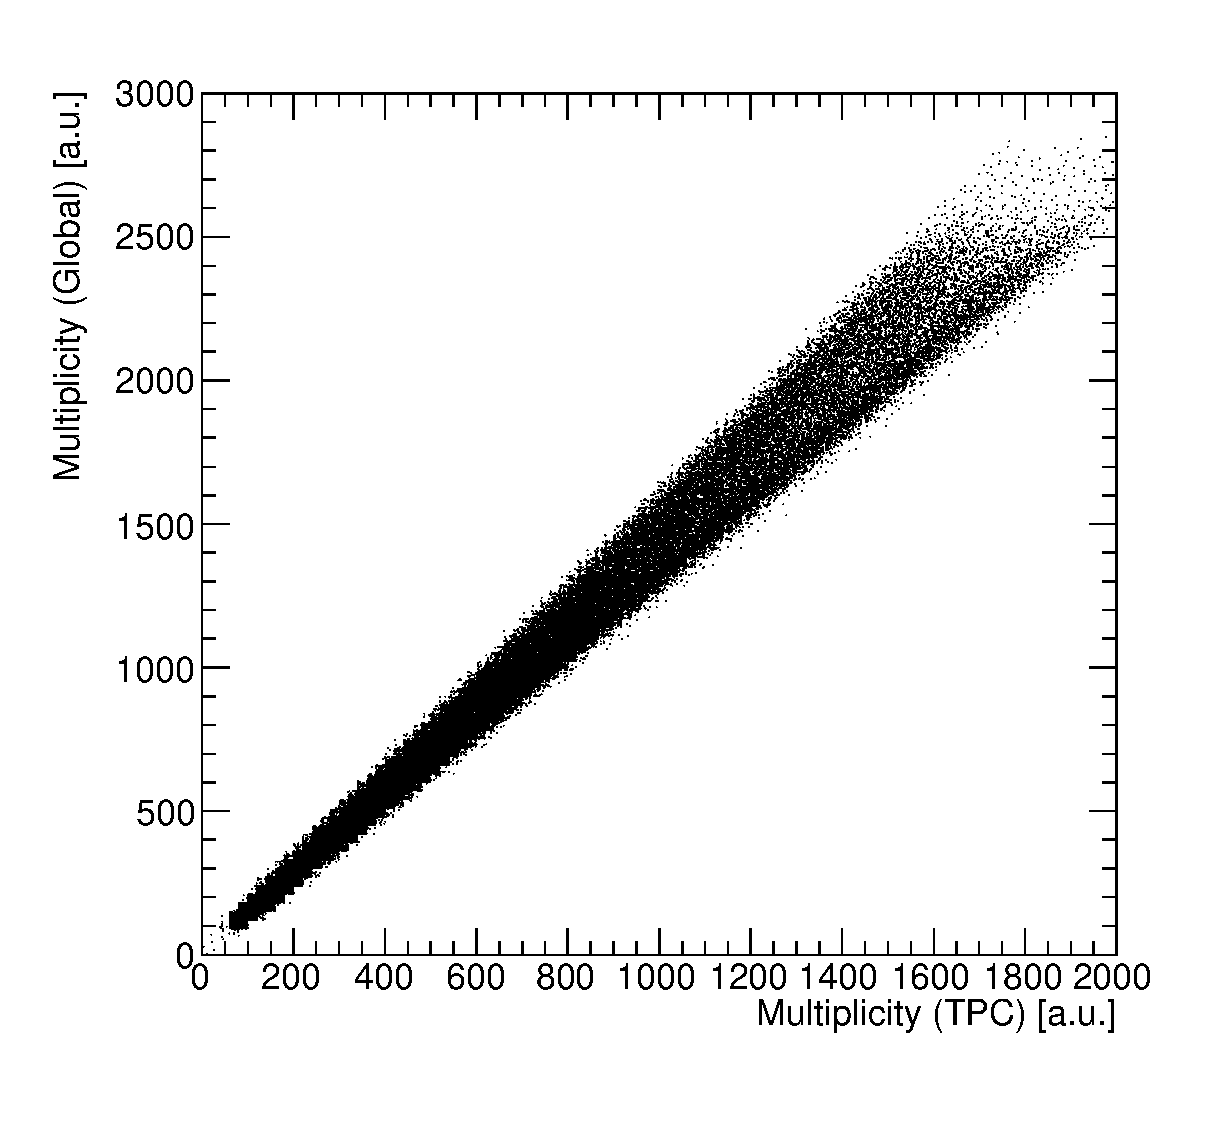
\includegraphics{figures/figs_systematics/outlier_on.eps}}
        \caption{The 2-dim distribution of TPC multiplicity and Global multiplicity. Left is the before exclude outlier(left) and right figure is after exclude outlier(right) events. }
        \label{fig:outlier}
        \end{center}   
     \end{figure}



\subsection{Systematics from Track selection}
	Following is the list of item for systematic uncertainty study form track selections.
	
\subsubsection{Track filter bit}
	As can see the Fig.\ref{fig:dndphi}, $\varphi$ flatness vary as track selection filter cuts, and it might affect the results of $SC(m,n)$ which is sensitive to $\phi$ distribution. This incompleteness of $\phi$ distribution comes from the limited precision with the detector performance. And each track filter cuts were evaluated by the thresholds on parameters used to select the tracks at the reconstruction level. Usually TPC only track cuts have relatively good(flat) $\phi$ distribution than GlobalSDD cut, but more fake and secondary tracks are included. Also GlobalSDD cut gives two small holes in $\phi$ distribution. 
			
 	\begin{figure}[h]
		\begin{center}
        	\resizebox{0.65\columnwidth}{!}{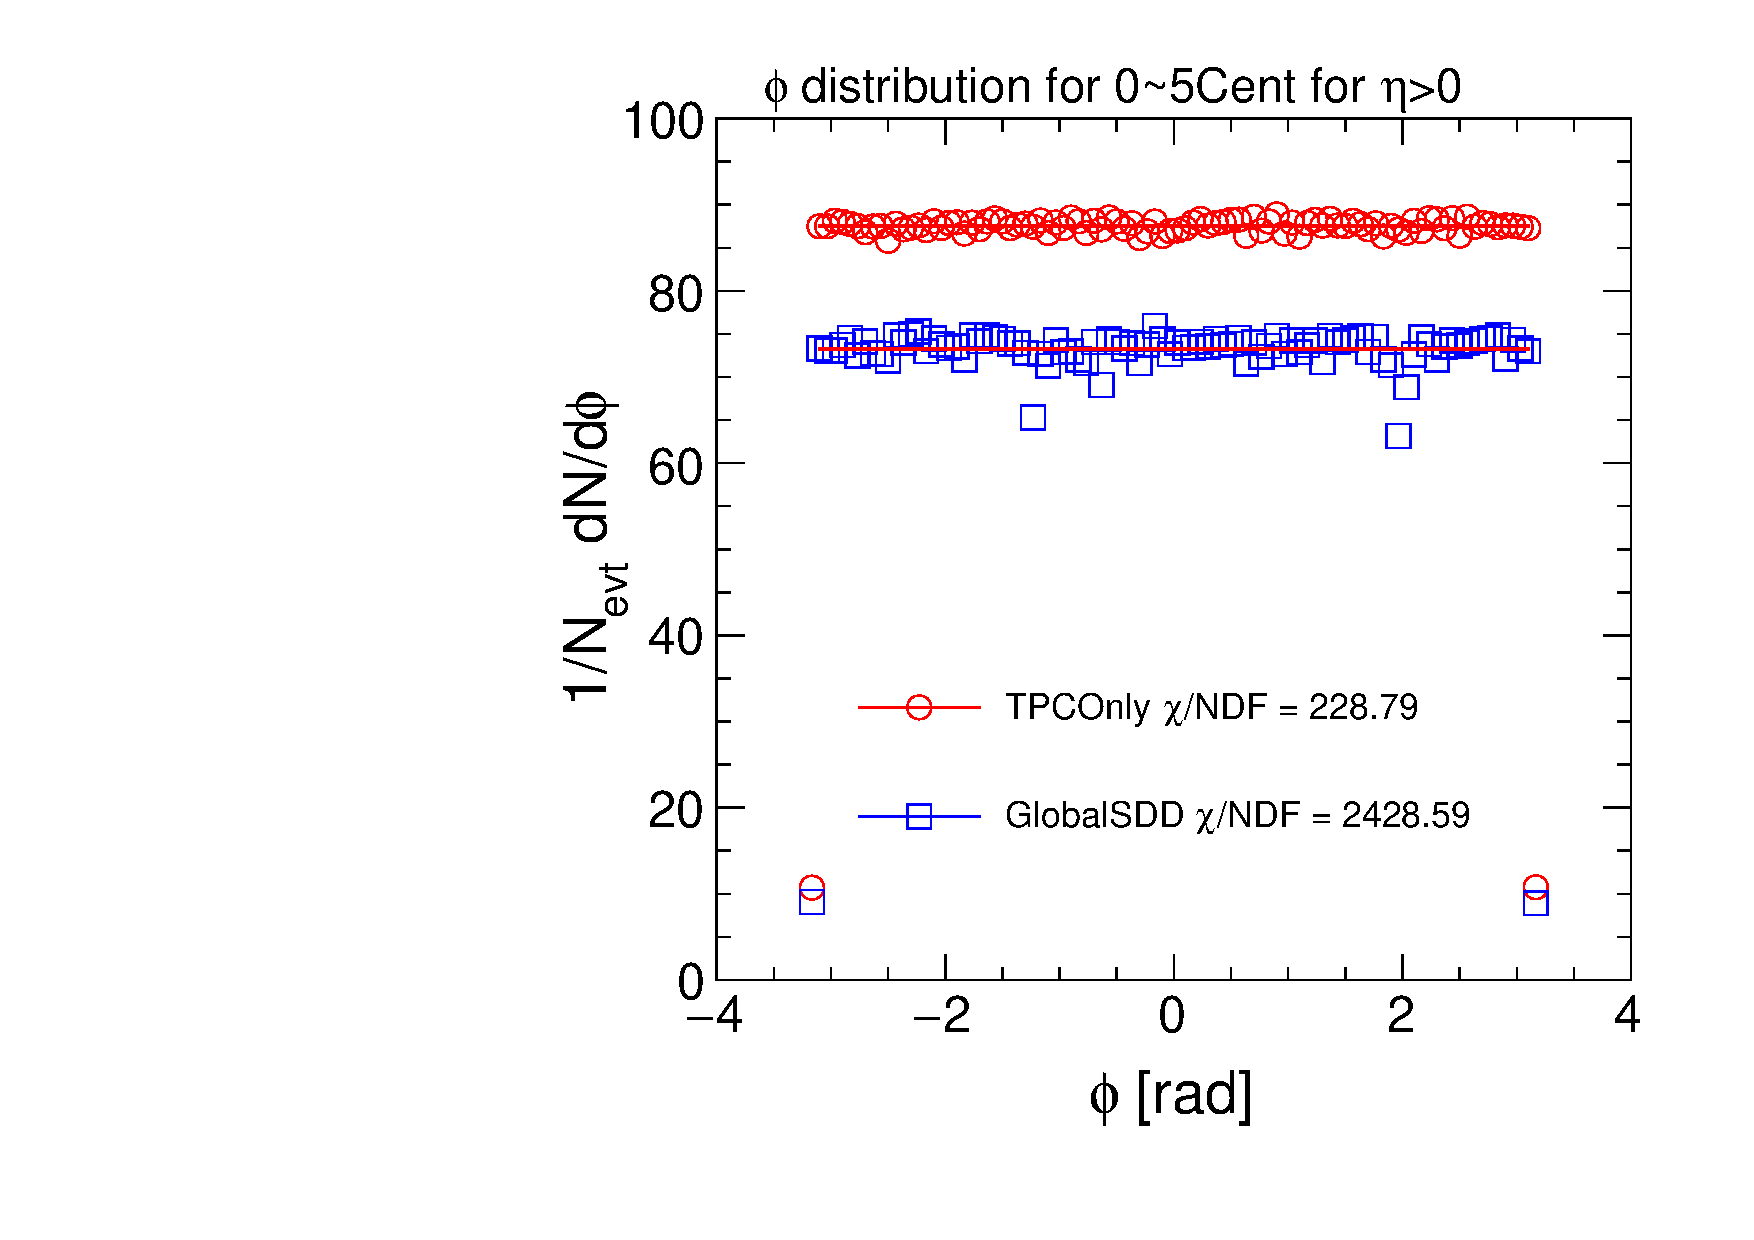
\includegraphics{figures/figs_systematics/dNdphi_TPCOnly_GlobalSDD_eta0_0}}
        \caption{$\chi/NDF$ of $dN/d\varphi$ distribution from ALICE LHC10h data with TPC only track selection filter and Global SDD filter.}
        \label{fig:dndphi}
        \end{center}   
     \end{figure}
	
\begin{table}[!h]
\begin{center}
\begin{tabular}{c|c|l}
\hline
cut		  & filter bit    & comments \\ \hline
TPCOnly   & 128 ( 7 )     & GetStandardTPCOnlyTrackCuts() \\
	      &               & + SetMinNClustersTPC(70)\\ \hline
GlobalSDD & 96  ( 5$|$6)  & GetStandardITSTPCTrackCuts2010()  \\ 
	      &               & with requiring the first SDD cluster \\ 
	      &               & instead of an SPD cluster \\ \hline
\end{tabular}
\caption{ALICE Track selection filter conditions}
\end{center}
\end{table}

To estimate systematic uncertainty from the track selection filter cut, we measure the results from different track selections and compare with the default setting.
	
	
\subsubsection{Charge combination}

We used 4p- and 2p- correlation to measure $SC(m,n)$. The multiparticle cumulants are expected to remove non-flow effect by cancellation each other, however it is hard to prove there is perfectly absense of non-flow effects in $SC(m,n)$. To estimate remain non-flow effects, such as re-reinteraction with other particles in the system after leaving the domain, the modification of the jet-like two-particle correlations, resonance decays, and final state interactions (particularly Coulomb effects).  Such flowing cluster contributes to cumulants by definition as being genuine four particle correlations, however, due to charge conservation, we will have in the cluster always particles of opposite charge. Therefore, by performing an independent analysis only with like-sign charges, we are estimating the contribution from flowing clusters. 



\subsubsection{Efficiency correction}

The correction to $p_T$ dependent efficiency were also tested, and taken into systematic uncertainty. Because of incompleteness of track reconstruction, correction steps are necessary to trace back from reconstructed tracks to the orignally generated particles from the collisions. Usually this study were conducted with a Monte Carlo simulation such as HIJING for Pb+Pb coliisions and PYTHIA for the $p$-$p$ collisions. The single track reconstruction efficiency, and contamination form the secondary particles were shown in FIg.\ref{fig:eff}

		
 	\begin{figure}[!p]
		\begin{center}
        	\resizebox{0.65\columnwidth}{!}{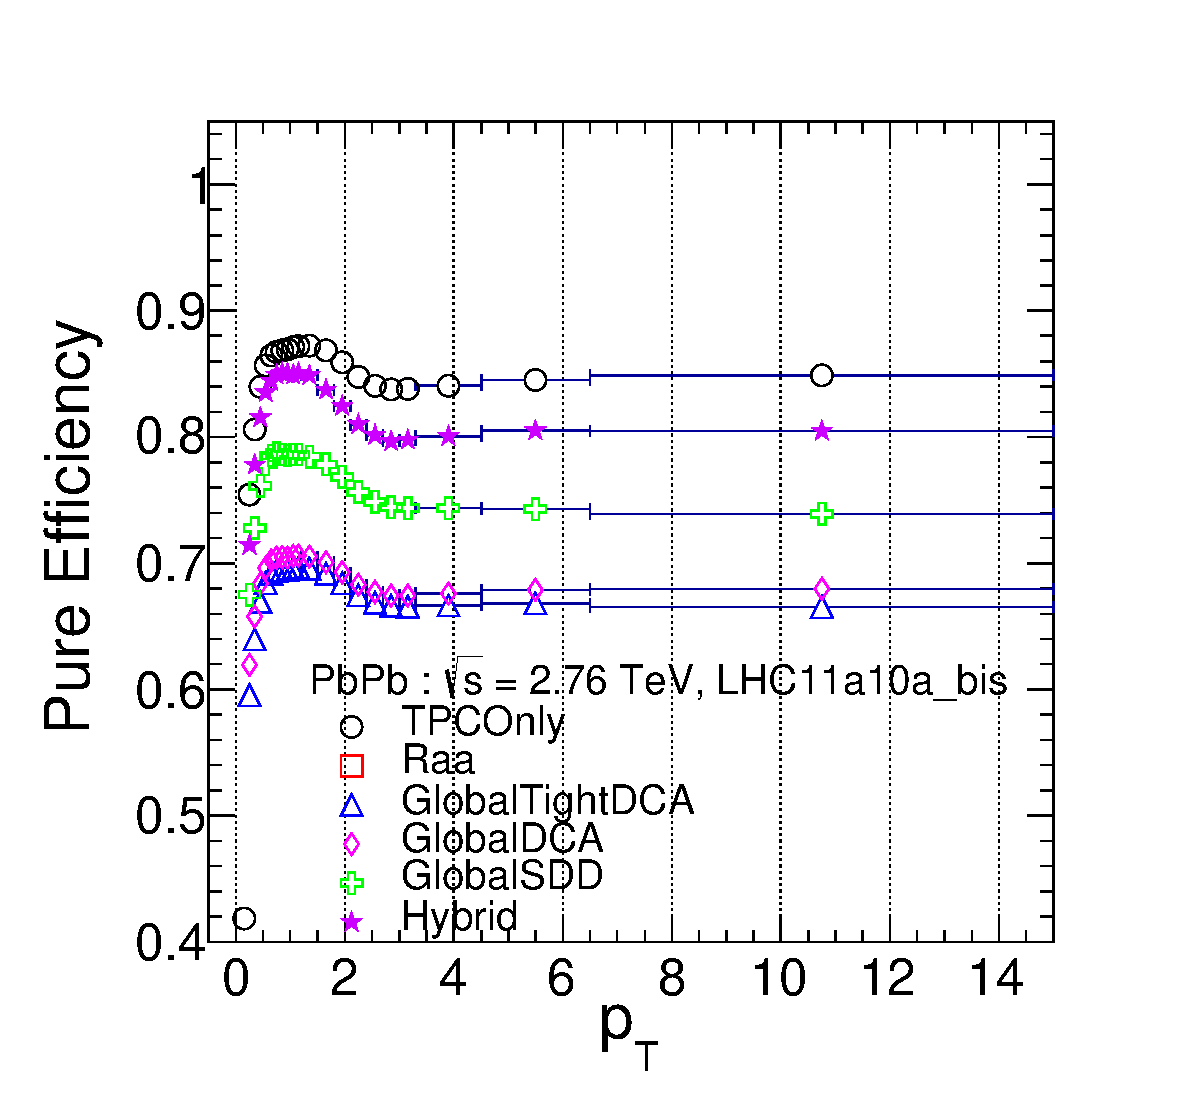
\includegraphics{figures/figs_systematics/PureEfficiency_PbPb276}}
        	\resizebox{0.65\columnwidth}{!}{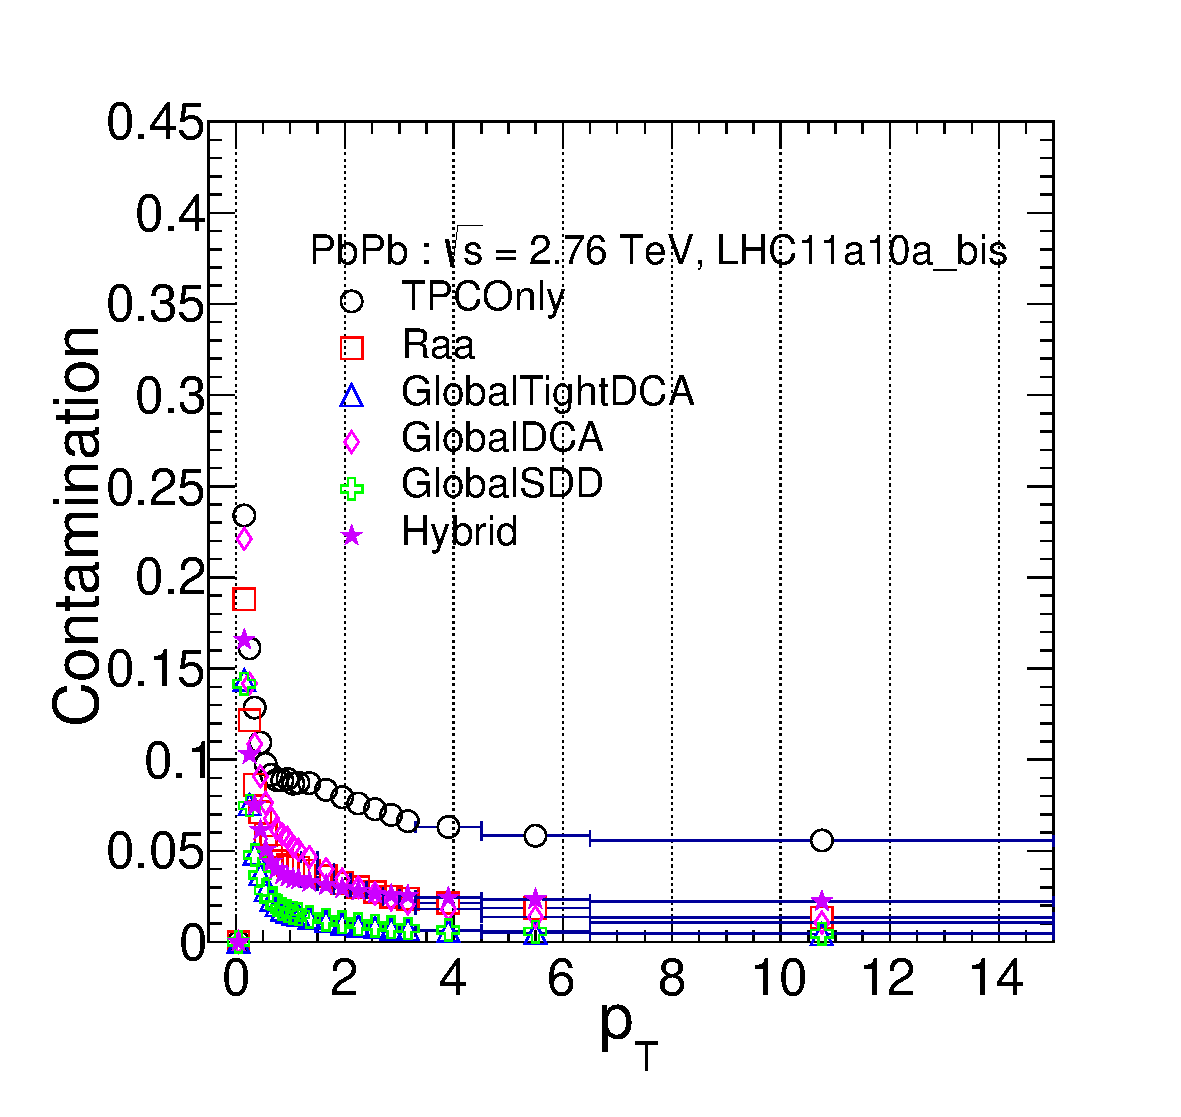
\includegraphics{figures/figs_systematics/Contamination_PbPb276}}
        \caption{Tracking efficiency of single particle reconstruction as a function of $p_T$ (left) and contamination of single particle as a function of $p_T$ (right) for ALICE with various track selection filter}
        \label{fig:eff}
        \end{center}   
     \end{figure}



\subsection{Overall systematic uncertainty}

All systematic uncertainty checks discussed in this analysis were included in the final systematic uncertainty. All individual checks are performed independently and these all systematics were combined in quadrature to obtain the final uncertainty. The tabulated systematic uncertainties are listed below tables.

\begin{table}[!p]
\begin{tabular}{c|c|c|c|c|c}
 
  Type  [\%]						&   SC(3,2)   &  SC(4,2) & SC(5,2) & SC(5,3) & SC(4,3)\\   \hline  \hline
  Non-uniform $\phi$ distribution	& $<1$	& 1.2	&9.5 	&17.3	&11.3	  	\\ \hline
  Track filter bit selection 		& 8.4	& 4.9	&9.1	&9.1		&11.9	 	\\ \hline
  Efficiency correction				& 3.1	& 4.4	&1.5	&1.7		&1.3	 \\ \hline
  Z-vertex cut						& 2.1	& 1.5	&2.1	&1.9		&3.0	\\ \hline
  Charge combination				& 4.5	& 12.1	&18.5	&19.5	&6.8 	\\ \hline
  high multiplicity outliers			& $<1$	& 2		&2.1	&2.1		&$<1$	\\ \hline
  Magnetic field polarization		& 2.1	& 2.7	&1.3	&1.5		&1.1	 \\ \hline   
  Centrality determination			& $<1$	& $<1$	&3.1	&7.6		&1.5 	\\ \hline   \hline
  Overall 							& 10.8	& 17.9	&22.8	&28.8	&18.4
  
\end{tabular}
\caption{Systematic uncertainties of $SC(m,n)$. Overall systematics are quadratically merged results of each individual systematic error}
\end{table}

\begin{table}[!p]
\begin{tabular}{c|c|c|c|c|c}
 
  Type  [\%]						&   NSC(3,2)   &  NSC(4,2) & NSC(5,2) & NSC(5,3) & NSC(4,3)\\   \hline  \hline
  Non-uniform $\phi$ distribution	& $<1$	& 1.1	&7.5 	&15.3	&12.4	  	\\ \hline
  Track filter bit selection 		& 7.3	& 4.9	&8.4	&12.1	&11.1	 	\\ \hline
  Efficiency correction				& 3.1	& 3.4	&1.5	&1.7		&1.3	 \\ \hline
  Z-vertex cut						& 2.1	& 1.5	&2.1	&1.9		&3.0		\\ \hline
  Charge combination				& 2.3	& 5.1	&18.2	&19.5	&6.1 	\\ \hline
  high multiplicity outliers			& $<1$	& 2		&2.1	&3.1		&$<1$	\\ \hline
  Magnetic field polarization		& 2.1	& 2.7	&3.6	&5.1		&4.1	 \\ \hline   
  Centrality determination			& $<1$	& $<1$	&1.4	&1.5		&$<1$ 	\\ \hline   \hline
  Overall 							& 9.1	& 8.1	&22.2	&28.3	&18.5
  
\end{tabular}
\caption{Systematic uncertainties of $NSC(m,n)$. Overall systematics are quadratically merged results of each individual systematic error}
\end{table}


